% =====================================================================
% Complete Figure Example: Skeleton C — Central Hero + 4 Panels
% =====================================================================
% USAGE: Complete compilable template. Uses explicit (x,y,w,h) for
% each zone — NO fit library (which has zone-outside trap).
%
% LAYOUT GRID (exact positions):
%   Title:           y=[10.0, 11.0]   x=[0, 21]
%   LU Hyperparams:  x=[0.0,  9.5]    y=[6.0, 9.5]   teal
%   RU Benchmarks:   x=[11.0, 21.0]   y=[6.0, 9.5]   blue
%   HERO Central:    x=[0.0,  21.0]   y=[1.5, 5.5]   purple
%   LD Pipeline:     x=[0.0,  9.5]    y=[-2.5, 1.0]  gold
%   RD Metrics:      x=[11.0, 21.0]   y=[-2.5, 1.0]  green
%   Legend:          x=[0, 21]        y=[-3.5, -3.0]
%
% Sub-agent: replace titles + labels + numbers. Keep grid + zone rects.
% =====================================================================

\documentclass[tikz,border=15pt]{standalone}
\usepackage{xcolor,tikz,amsmath,amssymb}
\usetikzlibrary{positioning,calc,backgrounds,arrows.meta,bending}

\definecolor{acaBlueLine}{HTML}{3060A8}
\definecolor{acaBlueFill}{HTML}{6890C8}
\definecolor{acaBlueBg}{HTML}{DCE6F4}
\definecolor{acaPurpleLine}{HTML}{6E3FA0}
\definecolor{acaPurpleBg}{HTML}{EDE3F6}
\definecolor{acaOrangeLine}{HTML}{D06020}
\definecolor{acaGreenLine}{HTML}{389050}
\definecolor{acaTealLine}{HTML}{1F8F8F}
\definecolor{acaTealBg}{HTML}{D3EBEB}
\definecolor{acaGoldLine}{HTML}{B08820}
\definecolor{acaGoldBg}{HTML}{F4E8CC}
\definecolor{acaGreyLine}{HTML}{606060}
\definecolor{cellLo}{HTML}{F0E8F8}
\definecolor{cellHi}{HTML}{6E3FA0}

\pgfdeclarelayer{background}
\pgfsetlayers{background,main}

\tikzset{
  base box/.style={
    rectangle, rounded corners=3pt, line width=0.5pt,
    minimum height=0.55cm, font=\scriptsize, align=center, inner sep=3pt,
  },
}

% Helper: draw zone bg + border + title strip
\newcommand{\drawzone}[6]{
  % #1=line color, #2=bg color, #3=x0, #4=y0, #5=x1, #6=y1
  \begin{pgfonlayer}{background}
    \fill[#2!50, rounded corners=4pt] (#3, #4) rectangle (#5, #6);
  \end{pgfonlayer}
  \draw[#1, line width=0.7pt, rounded corners=4pt]
    (#3, #4) rectangle (#5, #6);
}

\newcommand{\zonetitle}[5]{
  % #1=color #2=x0 #3=x1 #4=y_top #5=title
  \pgfmathsetmacro\titleX{(#2 + #3) / 2}
  \node[anchor=north, font=\small\bfseries, fill=#1, text=white,
        rounded corners=2pt, inner sep=3pt, inner ysep=2pt]
    at (\titleX, #4 - 0.15) {#5};
}

\begin{document}
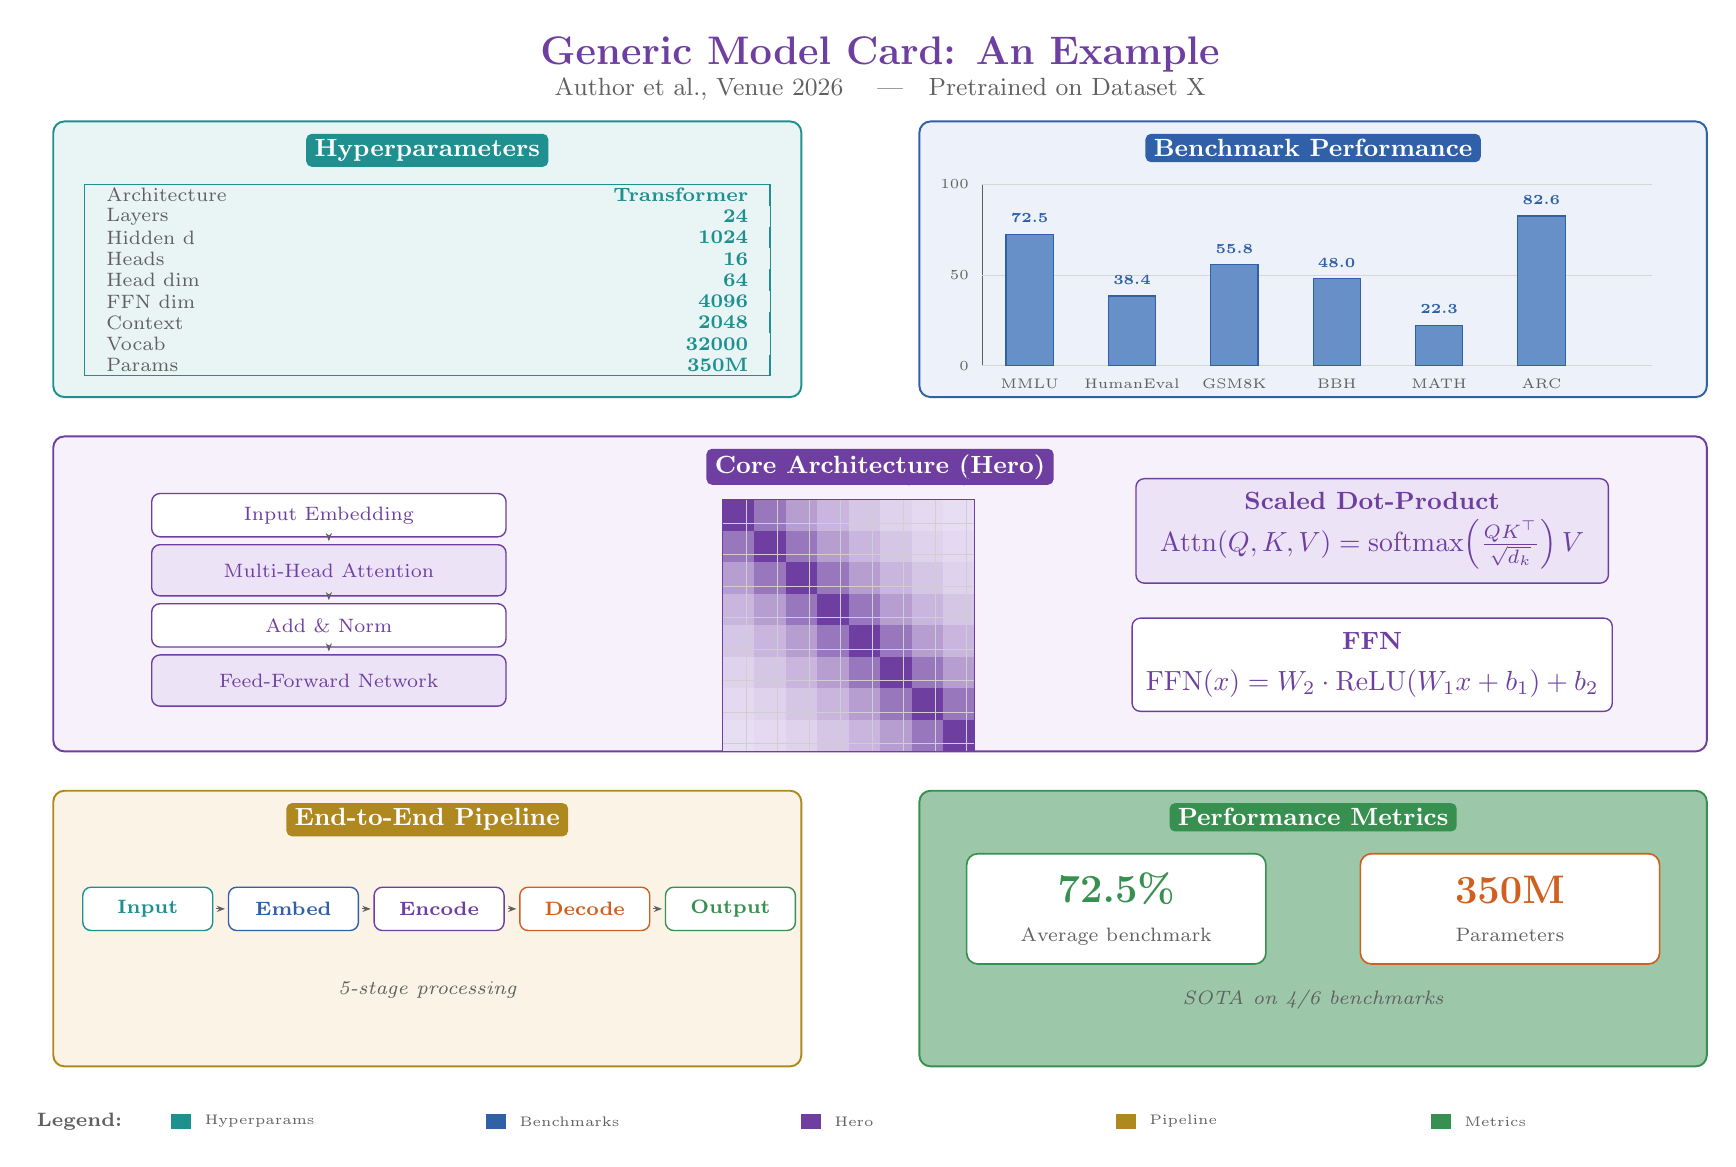
\begin{tikzpicture}

% =====================================================================
% TITLE
% =====================================================================
\node[font=\Large\bfseries, color=acaPurpleLine, anchor=south]
  at (10.5, 10.0) {Generic Model Card: An Example};
\node[font=\small, color=acaGreyLine, anchor=south]
  at (10.5, 9.65) {Author et al., Venue 2026 \quad|\quad Pretrained on Dataset X};

% =====================================================================
% LU PANEL: Hyperparameters table — x=[0, 9.5], y=[6, 9.5]
% =====================================================================
\drawzone{acaTealLine}{acaTealBg}{0}{6.0}{9.5}{9.5}
\zonetitle{acaTealLine}{0}{9.5}{9.5}{Hyperparameters}

% Table at x=[0.4, 9.1], y=[6.3, 8.7]
\def\xLU{0.4}\def\yLU{8.7}\def\rowH{0.27}\def\colW{8.7}
\def\tabdata{%
  Architecture/Transformer,%
  Layers/24,%
  Hidden d/1024,%
  Heads/16,%
  Head dim/64,%
  FFN dim/4096,%
  Context/2048,%
  Vocab/32000,%
  Params/350M%
}
\newcount\rowcount \rowcount=0
\foreach \k/\v in \tabdata { \global\advance\rowcount by 1 }
\edef\nrows{\the\rowcount}
\pgfmathsetmacro\tabH{\nrows * \rowH}
\draw[acaTealLine, line width=0.5pt]
  (\xLU, \yLU - \tabH) rectangle (\xLU + \colW, \yLU);
\foreach [count=\idx] \k/\v in \tabdata {
  \pgfmathsetmacro\ypos{\yLU - (\idx - 1) * \rowH}
  \pgfmathsetmacro\altfill{int(mod(\idx,2))}
  \ifnum\altfill=0
    \fill[acaTealBg!50] (\xLU, \ypos - \rowH) rectangle (\xLU + \colW, \ypos);
  \fi
  \node[anchor=west, font=\scriptsize, color=acaGreyLine]
    at (\xLU + 0.15, \ypos - \rowH/2) {\k};
  \node[anchor=east, font=\scriptsize\bfseries, color=acaTealLine]
    at (\xLU + \colW - 0.15, \ypos - \rowH/2) {\v};
}

% =====================================================================
% RU PANEL: Benchmark bar chart — x=[11, 21], y=[6, 9.5]
% =====================================================================
\drawzone{acaBlueLine}{acaBlueBg}{11.0}{6.0}{21.0}{9.5}
\zonetitle{acaBlueLine}{11}{21}{9.5}{Benchmark Performance}

% Chart at x=[11.8, 20.5], y=[6.3, 8.7]
\def\xBC{11.8}\def\yBC{6.4}\def\bcW{8.5}\def\bcH{2.3}
\draw[acaGreyLine, line width=0.4pt] (\xBC, \yBC) -- (\xBC + \bcW, \yBC);
\draw[acaGreyLine, line width=0.4pt] (\xBC, \yBC) -- (\xBC, \yBC + \bcH);
\foreach \pct in {0, 50, 100} {
  \pgfmathsetmacro\ypos{\yBC + \bcH * \pct / 100}
  \draw[acaGreyLine!25, line width=0.2pt]
    (\xBC, \ypos) -- (\xBC + \bcW, \ypos);
  \node[anchor=east, font=\tiny, color=acaGreyLine]
    at (\xBC - 0.05, \ypos) {\pct};
}

% 6 bars at fixed x positions (hard-code to avoid foreach quirks)
% bar width 0.6, gap 0.8, total = 6*0.6 + 5*0.8 = 7.6 cm → 8.5 cm chart, padding OK
\foreach \i/\name/\val in {1/MMLU/72.5, 2/HumanEval/38.4, 3/GSM8K/55.8,
                          4/BBH/48.0, 5/MATH/22.3, 6/ARC/82.6} {
  \pgfmathsetmacro\cx{\xBC + 0.6 + (\i - 1) * 1.3}
  \pgfmathsetmacro\bh{\bcH * \val / 100}
  \pgfmathsetmacro\bxL{\cx - 0.3}
  \pgfmathsetmacro\bxR{\cx + 0.3}
  \pgfmathsetmacro\btop{\yBC + \bh}
  \fill[acaBlueFill] (\bxL, \yBC) rectangle (\bxR, \btop);
  \draw[acaBlueLine, line width=0.4pt] (\bxL, \yBC) rectangle (\bxR, \btop);
  \node[font=\tiny\bfseries, color=acaBlueLine, anchor=south]
    at (\cx, \btop + 0.02) {\val};
  \node[font=\tiny, color=acaGreyLine, anchor=north]
    at (\cx, \yBC - 0.05) {\name};
}

% =====================================================================
% HERO CENTRAL ZONE: x=[0, 21], y=[1.5, 5.5]
% =====================================================================
\drawzone{acaPurpleLine}{acaPurpleBg}{0}{1.5}{21.0}{5.5}
\zonetitle{acaPurpleLine}{0}{21}{5.5}{Core Architecture (Hero)}

% Hero internal: 3 zones
% Left: sub-module stack at x=[1, 6]
\node[base box, fill=white, draw=acaPurpleLine, text=acaPurpleLine,
      minimum width=4.5cm] (h1) at (3.5, 4.5) {Input Embedding};
\node[base box, fill=acaPurpleBg, draw=acaPurpleLine, text=acaPurpleLine,
      minimum width=4.5cm, minimum height=0.65cm] (h2) at (3.5, 3.8)
  {Multi-Head Attention};
\node[base box, fill=white, draw=acaPurpleLine, text=acaPurpleLine,
      minimum width=4.5cm] (h3) at (3.5, 3.1) {Add \& Norm};
\node[base box, fill=acaPurpleBg, draw=acaPurpleLine, text=acaPurpleLine,
      minimum width=4.5cm, minimum height=0.65cm] (h4) at (3.5, 2.4)
  {Feed-Forward Network};
\foreach \a/\b in {h1/h2, h2/h3, h3/h4} {
  \draw[-{Stealth[length=3pt]}, line width=0.4pt, color=acaGreyLine,
        shorten >=1pt, shorten <=1pt]
    (\a.south) -- (\b.north);
}

% Middle: attention heatmap at x=[8.5, 12.5]
\def\xH{8.5}\def\yH{4.7}\def\cs{0.4}\def\N{8}
\foreach \i in {1,...,\N} {
  \foreach \j in {1,...,\N} {
    \pgfmathsetmacro\val{exp(-abs(\i-\j)/2.5)*100}
    \pgfmathsetmacro\val{int(\val)}
    \pgfmathsetmacro\cx{\xH + (\j - 0.5) * \cs}
    \pgfmathsetmacro\cy{\yH - (\i - 0.5) * \cs}
    \fill[cellHi!\val!cellLo]
      (\cx - \cs/2, \cy - \cs/2) rectangle (\cx + \cs/2, \cy + \cs/2);
  }
}
\draw[step=\cs cm, acaGreyLine!30, line width=0.15pt]
  (\xH, \yH) grid (\xH + \N*\cs, \yH - \N*\cs);
\draw[acaPurpleLine, line width=0.5pt]
  (\xH, \yH) rectangle (\xH + \N*\cs, \yH - \N*\cs);
\node[font=\tiny\bfseries, color=acaPurpleLine, anchor=south]
  at (\xH + \N*\cs/2, \yH + 0.05) {Attention Weights ($N=8$)};

% Right: 2 formula boxes at x=[13.5, 20]
\node[rectangle, rounded corners=3pt, fill=acaPurpleBg,
      draw=acaPurpleLine, line width=0.5pt, inner sep=5pt,
      align=center, text=acaPurpleLine,
      minimum width=6.0cm]
  (form1) at (16.75, 4.3)
  {{\small\bfseries Scaled Dot-Product}\\[3pt]
   $\text{Attn}(Q,K,V) = \text{softmax}\!\left(\frac{QK^\top}{\sqrt{d_k}}\right) V$};
\node[rectangle, rounded corners=3pt, fill=white,
      draw=acaPurpleLine, line width=0.5pt, inner sep=5pt,
      align=center, text=acaPurpleLine,
      minimum width=6.0cm]
  (form2) at (16.75, 2.6)
  {{\small\bfseries FFN}\\[3pt]
   $\text{FFN}(x) = W_2 \cdot \text{ReLU}(W_1 x + b_1) + b_2$};

% =====================================================================
% LD PANEL: Pipeline — x=[0, 9.5], y=[-2.5, 1.0]
% =====================================================================
\drawzone{acaGoldLine}{acaGoldBg}{0}{-2.5}{9.5}{1.0}
\zonetitle{acaGoldLine}{0}{9.5}{1.0}{End-to-End Pipeline}

\foreach \i/\name/\col in {1/Input/acaTealLine, 2/Embed/acaBlueLine,
                          3/Encode/acaPurpleLine, 4/Decode/acaOrangeLine,
                          5/Output/acaGreenLine} {
  \pgfmathsetmacro\cx{0.6 + (\i - 1) * 1.85}
  \node[rectangle, rounded corners=3pt, fill=white, draw=\col,
        line width=0.5pt, font=\scriptsize\bfseries, text=\col,
        minimum width=1.65cm, minimum height=0.55cm]
    (pip\i) at (\cx + 0.6, -0.5) {\name};
}
\foreach \a/\b in {1/2, 2/3, 3/4, 4/5} {
  \draw[-{Stealth[length=3pt]}, line width=0.4pt, color=acaGreyLine,
        shorten >=1pt, shorten <=1pt]
    (pip\a.east) -- (pip\b.west);
}
\node[font=\scriptsize\itshape, color=acaGreyLine, anchor=north]
  at (4.75, -1.3) {5-stage processing};

% =====================================================================
% RD PANEL: Metric cards — x=[11, 21], y=[-2.5, 1.0]
% =====================================================================
\drawzone{acaGreenLine}{acaGreenLine}{11.0}{-2.5}{21.0}{1.0}
\zonetitle{acaGreenLine}{11}{21}{1.0}{Performance Metrics}

\node[draw=acaGreenLine, fill=white, rounded corners=4pt,
      line width=0.6pt, minimum width=3.8cm, minimum height=1.4cm,
      align=center, inner sep=5pt]
  at (13.5, -0.5)
  {{\Large\bfseries\color{acaGreenLine} 72.5\%}\\[2pt]
   {\scriptsize\color{acaGreyLine} Average benchmark}};
\node[draw=acaOrangeLine, fill=white, rounded corners=4pt,
      line width=0.6pt, minimum width=3.8cm, minimum height=1.4cm,
      align=center, inner sep=5pt]
  at (18.5, -0.5)
  {{\Large\bfseries\color{acaOrangeLine} 350M}\\[2pt]
   {\scriptsize\color{acaGreyLine} Parameters}};

\node[font=\scriptsize\itshape, color=acaGreyLine, anchor=north]
  at (16, -1.4) {SOTA on 4/6 benchmarks};

% =====================================================================
% BOTTOM-MOST: Color Legend strip — y=[-3.5, -3.0]
% =====================================================================
\node[font=\scriptsize\bfseries, color=acaGreyLine, anchor=east]
  at (1.0, -3.2) {Legend:};
\foreach \i/\col/\lab in {%
  1/acaTealLine/Hyperparams,%
  2/acaBlueLine/Benchmarks,%
  3/acaPurpleLine/Hero/Core,%
  4/acaGoldLine/Pipeline,%
  5/acaGreenLine/Metrics%
} {
  \pgfmathsetmacro\lx{1.5 + (\i - 1) * 4.0}
  \fill[\col] (\lx, -3.3) rectangle (\lx + 0.25, -3.1);
  \node[anchor=west, font=\tiny, color=acaGreyLine]
    at (\lx + 0.3, -3.2) {\lab};
}

\end{tikzpicture}
\end{document}
